% --- CÓDIGO ATUALIZADO para Analise/shell_sort_analise.tex ---

\subsubsection*{Análise e Interpretação dos Resultados - Shell Sort}

\qquad A análise exata do \textit{Shell Sort} é mais complexa que a dos demais algoritmos deste trabalho, pois seu desempenho depende diretamente da sequência de intervalos (\textit{gaps}) utilizada. A análise apresentada a seguir considera a implementação com a sequência $n/2, n/4, \dots, 1$ e se baseia nos resultados já estabelecidos na literatura \cite{sedgewick}.

\qquad Os principais casos de desempenho para essa sequência de \textit{gaps} são os seguintes:
\begin{itemize}
    \item \textbf{Melhor caso:} ocorre quando o vetor já está ordenado. O laço externo dos \textit{gaps} executa aproximadamente $\log n$ vezes e, como nenhum deslocamento é necessário, o laço interno percorre o vetor realizando apenas comparações. Isso resulta em complexidade $O(n \log n)$.

    \item \textbf{Pior caso:} para a sequência de \textit{gaps} utilizada no código, o pior caso conhecido é $O(n^2)$. Existem arranjos específicos de dados que levam o algoritmo a esse desempenho.

    \item \textbf{Caso médio:} não há uma fórmula fechada para essa sequência de \textit{gaps}. As estimativas mais aceitas indicam uma complexidade subquadrática, em torno de $O(n^{1,5})$. Na prática, o que importa é que o desempenho médio fica bem abaixo de $O(n^2)$.
\end{itemize}

\qquad Para ilustrar de forma concreta o funcionamento do algoritmo, a Figura \ref{fig:shell_teste_mesa} apresenta um teste de mesa realizado com essa mesma sequência de \textit{gaps}, mostrando passo a passo como o vetor se aproxima da ordenação a cada passagem.

% --- IMAGEM ÚNICA PARA A ANÁLISE GERAL ---
\begin{figure}[htbp]
    \centering
    % ATENÇÃO: Faça o upload da sua imagem do teste de mesa com este nome ou altere aqui
    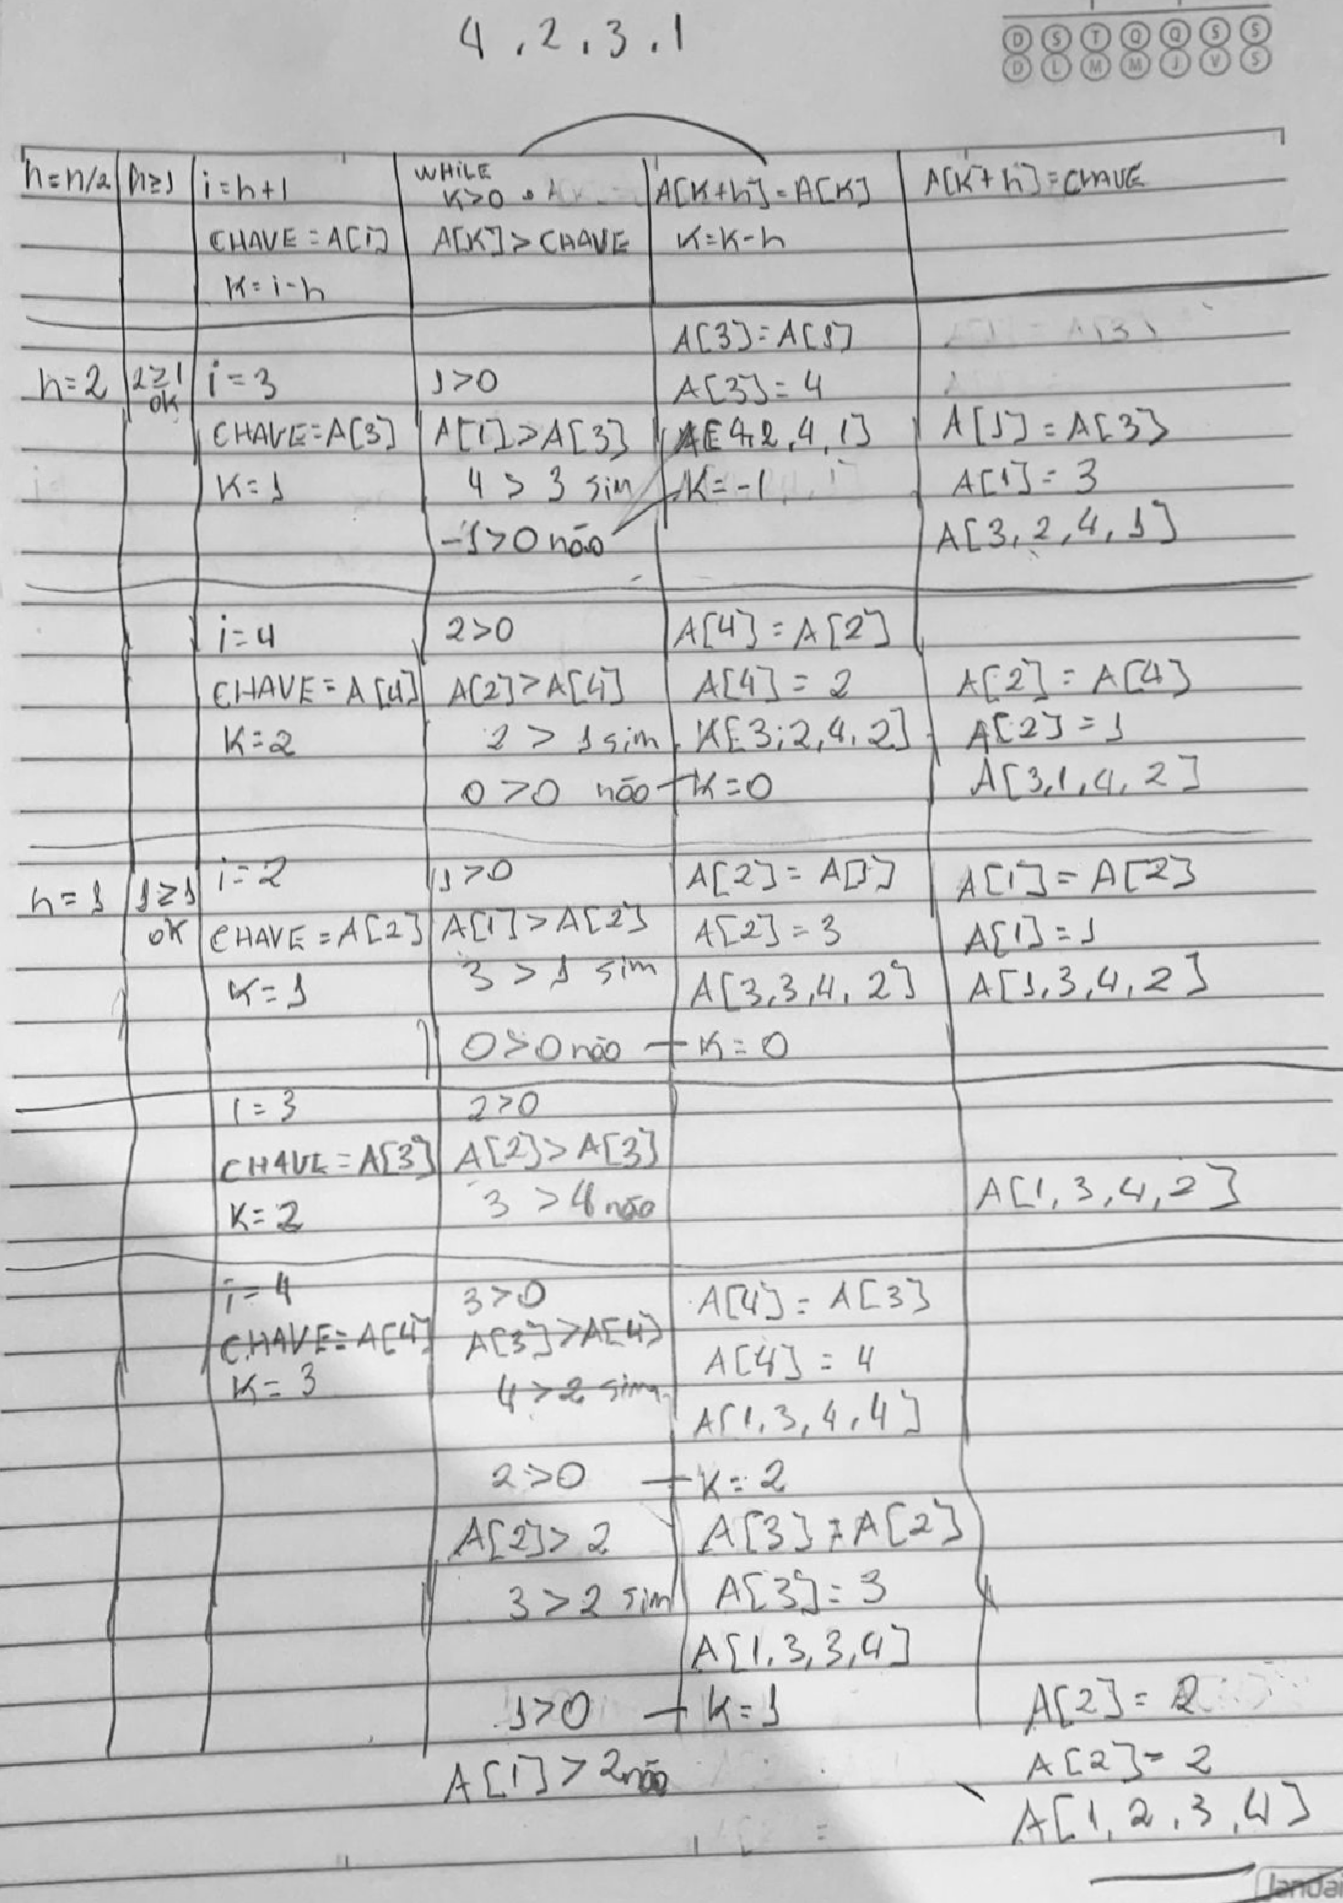
\includegraphics[width=0.9\textwidth]{Imagens/Shell_sort/TesteDeMesa.png}
    \caption{Teste de mesa do Shell Sort com a sequência de \textit{gaps} $n/2, n/4, \dots, 1$ (elaborado pelo autor).}
    \label{fig:shell_teste_mesa}
\end{figure}

\FloatBarrier

\qquad Os tempos medidos nos testes são compatíveis com essa análise: ao aumentar a entrada de 100.000 para 1.000.000 de elementos, o tempo do caso aleatório cresceu cerca de 15 vezes, enquanto em um algoritmo quadrático o crescimento esperado seria de aproximadamente 100 vezes.

\qquad Quanto à \textbf{complexidade de espaço}, o \textit{Shell Sort} apresenta complexidade $O(1)$, pois a ordenação é feita \textit{in-place}, sem uso de estruturas auxiliares proporcionais a $n$.